The value in the resampling process above largely lies in the ability to present well-defined document prototypes to a retrieval stage.  There are many potential sources for document retrieval according to this prototype, including the original input corpus, a separate `super-corpus', or, ideally a separate population (that is itself not a sample).

The proof-of-concept evaluated here implements a mechanism similar to that of BootCaT~\td{cite}, using a search engine to retrieve results based on key n-grams.  This mechanism was selected due to the pertinence of its method to other corpus building efforts --- there is no technical limitation imposed by the software tool, and users are free to select any other source of data or mechanism of retrieval.

The similarity of the retrieval system described here to BootCaT, along with the use of concrete prototype documents, allows us to inspect the `measurement error' of using search engines to retrieve data based on key terms.  This evaluation is, therefore, primarily a qualitative assessment of that bias and a preliminary assessment of its sources.

% ---

The retrieval process is performed iteratively using the components evaluated in the previous sections:

\begin{enumerate}
    \item Sample a prototype document from the corpus profile
    \item Retrieve candidate links using the Microsoft Bing web service~\footnote{\url{https://datamarket.azure.com/dataset/bing/searchweb}}.
    \item Download, remove boilerplate (using justext~\td{cite}), and classify each document using heuristics from the corpus profile.
    \item Measure distance in the resulting vector space according to each heuristic's value.
\end{enumerate}

This results in a collection that has at best a superset of the prototype selection's metadata.

For this evaluation, the written portions of the BNC were used as the seed corpus.  Keywords used for search were generated using log likelihood scores, and no cutoff was used: instead, the random selection algorithm was weighted by the resulting score.

The spoken and \texttt{w\_Misc} categories were omitted for a number of reasons.  Spoken data was omitted on the conjecture that it is difficult to find online~\footnote{Retrieval of transcriptions may be facilitated by searching for genre-specific features in addition to keywords, and this form of specialism is a potential avenue for improving the accuracy of all genres.}, leading to a predictable gap in the resulting corpus.  \texttt{W\_misc} was omitted due to the need for an accurate classification step, and because keyword-based retrieval requires that said keywords are highly representative of a given genre.  Both of these issues are potentially solvable in future work, yet lie outside the scope of this thesis.


The retriever must, as far as possible, retrieve documents according to \textsl{all} prototype metadata dimensions, that is, it must perform the equivalent to an agglomerative query.  This is a particular challenge for search engines due to their generality.  Since the Bing API lacks tools to filter by any of the three dimensions used in this evaluation, the primary focus was on genre --- word count and reading ease were both free to vary.  Language was specified as \texttt{en\_GB}.

% TODO: Write in discussion about how this is challenging but that a hybrid system might work best, say retrieve from scholar if it's a paper.








This process is deliberately agnostic of any internal variables: the \textsl{content} of the retrieved texts is also affected by the choice of retrieval mechanism, however, this is part of the variance desired in the dataset, and should form part of any motivating research question.

The problem of when the output corpus is `sufficiently large' may not be solved using this method: whilst the convergeance of the output corpus to the input is known to some degree of certainty, the same cannot be said of the errors in retrieval.  Assuming that each text is entirely accurate to its prototype will yield a corpus showing the same distribution as the input, but this does not mean that the source used is presenting data in an unbiased manner, or that sufficient variation has been captured to generalise about \textsl{that} population.

It is also possible to select documents that are not a perfect fit to the prototype: indeed, this may be necessary where continuous measures are used to characterise the sampling design.  In this case, the residual variation may be used to determine bias in the selection method by measuring how non-uniform the distribution of these residuals is.  Note, however, that even uniform nonzero residuals represent an overall increase in dispersion compared to the input distribution: it is almost certainly more useful to deliberately apply this to the input distribution by applying a smoothing method prior to resampling than it is to rely on the document retrieval stage (which may apply said dispersion in less predictable ways).

\til{
further work:\\
Though not implemented here, it is possible to use this known error distribution as a correction mechanism for the sampler, deliberately seeking to `shore up' the residuals.  This kind of feedback loop is used in bootstrapping algorithms such as Gibbs and slice sampling, though its application to a procedure based on a fairly hard-to-predict search mechanism (web search engines) presents major engineering challenges.
}

% --


\begin{figure}[Ht]
    % ./analysis/loglik-significance.r
    \centering
    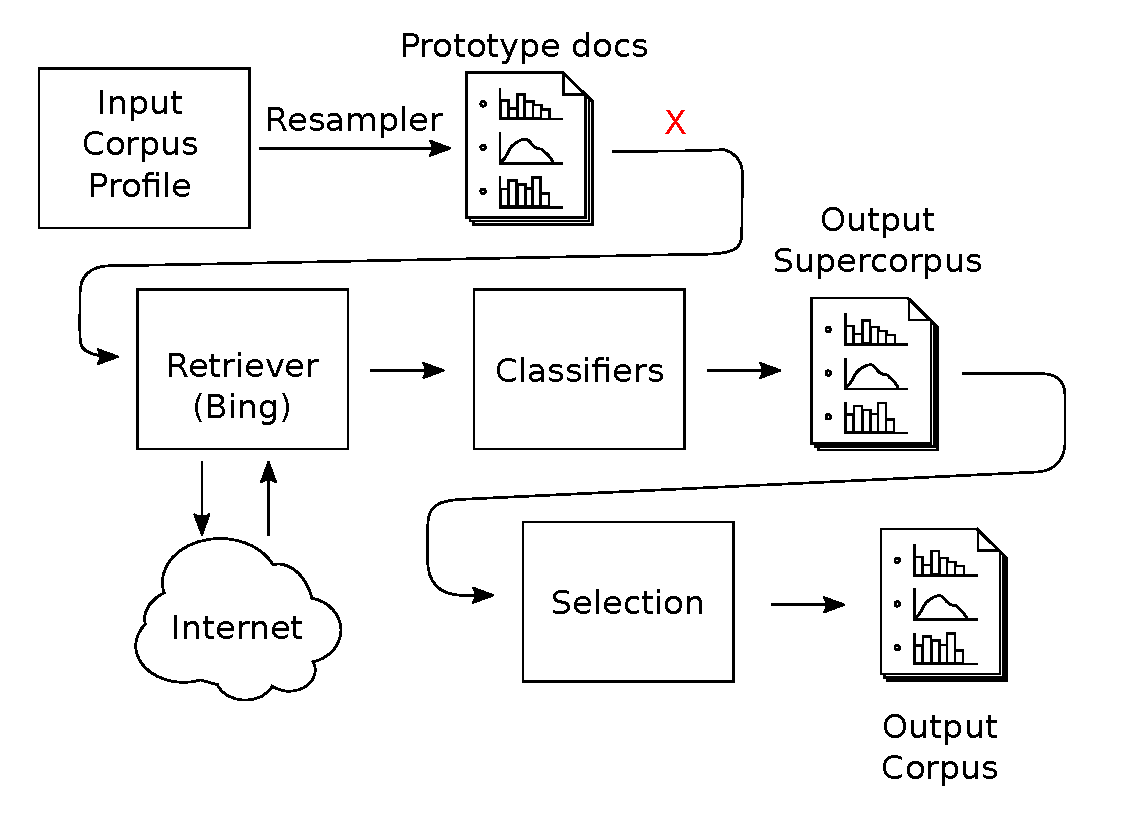
\includegraphics[width=0.8\textwidth]{evaluation/retrieval-overview}
    \caption{An overview of the retrieval mechanism used in the proof-of-concept implementation.}
    \label{fig:evaluation:retrieval:outline}
\end{figure}



The retrieval method used here (outlined in Chapter~\ref{sec:rebuilding} and Figure~\ref{fig:evaluation:retrieval:outline}) is based on the principle of heuristically seeking documents fitting the prototype, followed by a ranking stage and selection of the highest-ranked document.  This means that it has the potential to output imperfect documents but is maximally unlikely to do so.  It does not adjust for any accumulated error during execution, so has the potential to gradually accumulate errors in one particular direction if `perfectly matched' documents are not available within the parameters given.  This approach is largely taken to prevent the retriever from searching endlessly for a combination of metadata values that simply do not exist in the sources to which it has access: many specific uses of this technique will be able to use far more certain methods for their retrieval stage (up to and including manual selection of documents).



\subsection{Method}
\label{sec:evaluation:method}





\subsection{Data}
\label{sec:evaluation:method}
Discuss which corpora were chosen and why

\subsection{Results}
\label{sec:evaluation:}
Provide quantitative measures for the two evaluation methods
%#\subsubsection{Partial/white box}
%Show how well classifiers and heuristics behave
\subsubsection{Complete/black box}
Show how well the whole system works

